%=======================================================================
%  Ten Key Figures --- a guided visual summary
%
%  Built by generate_key_figures.py. Figures are the same vector PDFs
%  the dissertation uses; numbers are injected from generated/numbers.tex.
%=======================================================================
\documentclass[11pt,a4paper]{article}

\usepackage[T1]{fontenc}
\usepackage[utf8]{inputenc}
\usepackage{mathptmx}
\usepackage[scaled=0.88]{helvet}
\usepackage{amsmath,amssymb}
\usepackage[margin=2.2cm,top=2.4cm,bottom=2.2cm]{geometry}
\usepackage{graphicx}
\usepackage{booktabs}
\usepackage{float}
\usepackage{xcolor}
\usepackage{enumitem}
\usepackage{microtype}
\usepackage{fancyhdr}
\usepackage{titlesec}
\usepackage[font=small,labelfont=bf,labelsep=period]{caption}
\usepackage{tcolorbox}
\tcbuselibrary{skins}
\usepackage[hidelinks]{hyperref}

\definecolor{accent}{HTML}{0072B2}
\definecolor{warm}{HTML}{D55E00}
\definecolor{inkmuted}{HTML}{4D4D4D}
\definecolor{rule}{HTML}{BFBFBF}
\definecolor{panel}{HTML}{F4F7FA}
\definecolor{warmpanel}{HTML}{FDF3EC}

\hypersetup{colorlinks=true, linkcolor=accent, urlcolor=accent, linktoc=all,
            pdftitle={Blockchain-Based Electronic Voting: Ten Key Figures},
            pdfsubject={MSc Computing Science dissertation --- visual summary}}

\titleformat{\section}{\normalfont\sffamily\large\bfseries}{\thesection.}{0.6em}{}
\titlespacing*{\section}{0pt}{4pt}{8pt}

\pagestyle{fancy}
\fancyhf{}
\renewcommand{\headrulewidth}{0.4pt}
\fancyhead[L]{\footnotesize\sffamily\color{inkmuted}Ten Key Figures}
\fancyhead[R]{\footnotesize\sffamily\color{inkmuted}\thepage}

\setlength{\parskip}{0.35em}
\setlength{\parindent}{0pt}

%--- the explanation block --------------------------------------------
\newtcolorbox{readbox}{colback=panel, colframe=accent, boxrule=0pt,
  leftrule=2.4pt, arc=1pt, left=8pt, right=8pt, top=6pt, bottom=6pt,
  fontupper=\small}

\newtcolorbox{numberbox}{colback=warmpanel, colframe=warm, boxrule=0pt,
  leftrule=2.4pt, arc=1pt, left=8pt, right=8pt, top=5pt, bottom=5pt,
  fontupper=\small}

\newcommand{\lookat}[1]{\textsf{\bfseries\footnotesize WHAT YOU ARE LOOKING AT}\ \ #1\par\smallskip}
\newcommand{\shows}[1]{\textsf{\bfseries\footnotesize WHAT IT SHOWS}\ \ #1\par\smallskip}
\newcommand{\matters}[1]{\textsf{\bfseries\footnotesize WHY IT MATTERS}\ \ #1}
\newcommand{\keynumber}[1]{\textsf{\bfseries\footnotesize THE NUMBER TO REMEMBER}\ \ #1}

\newcommand{\Prob}{\mathbb{P}}
\newcommand{\Ex}{\mathbb{E}}
\newcommand{\Uv}{U_{v}}

% Generated by generate_report.py -- do not edit by hand.
% Every value here is read from results/ output.

\newcommand{\BallotCeilingPct}{30}
\newcommand{\BallotCostRatio}{15}
\newcommand{\BallotStuffingAbsReduction}{0.325}
\newcommand{\BallotStuffingAcceptedBaseline}{0.498}
\newcommand{\BallotStuffingAcceptedProtected}{0.253}
\newcommand{\BallotStuffingBaseline}{0.442}
\newcommand{\BallotStuffingBaselineMedian}{0.0000}
\newcommand{\BallotStuffingBaselineStd}{0.487}
\newcommand{\BallotStuffingCIHigh}{0.343}
\newcommand{\BallotStuffingCILow}{0.308}
\newcommand{\BallotStuffingChernoffGap}{0.0216}
\newcommand{\BallotStuffingChernoffHolds}{100.0}
\newcommand{\BallotStuffingChernoffValid}{3,604}
\newcommand{\BallotStuffingIntervalWidth}{0.043}
\newcommand{\BallotStuffingMCError}{3.94e-4}
\newcommand{\BallotStuffingMCMaxError}{0.0230}
\newcommand{\BallotStuffingProtected}{0.116}
\newcommand{\BallotStuffingRelReduction}{73.7}
\newcommand{\BestPureMax}{0.423}
\newcommand{\BestPureMeanBaseline}{0.277}
\newcommand{\BestPureMin}{0.316}
\newcommand{\BestPureViableCount}{4}
\newcommand{\BriberyAbsReduction}{0.287}
\newcommand{\BriberyBaseline}{0.350}
\newcommand{\BriberyBaselineMedian}{0.0000}
\newcommand{\BriberyBaselineStd}{0.474}
\newcommand{\BriberyCIHigh}{0.304}
\newcommand{\BriberyCILow}{0.269}
\newcommand{\BriberyChernoffGap}{0.0423}
\newcommand{\BriberyChernoffHolds}{100.0}
\newcommand{\BriberyChernoffValid}{1,088}
\newcommand{\BriberyIntervalWidth}{0.018}
\newcommand{\BriberyMCError}{7.98e-5}
\newcommand{\BriberyMCMaxError}{0.0149}
\newcommand{\BriberyProtected}{0.064}
\newcommand{\BriberyRelReduction}{81.9}
\newcommand{\CertificationEpsilon}{10^{-3}}
\newcommand{\ChainIntegrityHeld}{never violated}
\newcommand{\CoalitionBetterCount}{4}
\newcommand{\CoalitionMeanBaseline}{0.800}
\newcommand{\CoalitionMeanGain}{0.522}
\newcommand{\CoalitionMeanProtected}{0.000}
\newcommand{\CoalitionScenarioCount}{5}
\newcommand{\ConvergenceFinalError}{0.0018}
\newcommand{\ConvergenceMaxSize}{50,000}
\newcommand{\ConvergenceMinSize}{10}
\newcommand{\ConvergenceSettles}{3,000}
\newcommand{\ConvergenceTolerance}{0.01}
\newcommand{\CriticalDetectionBindingCount}{4}
\newcommand{\CriticalDetectionMax}{0.118}
\newcommand{\CriticalDetectionMin}{0.050}
\newcommand{\ElectionTrials}{300}
\newcommand{\ElectorateMax}{4,999}
\newcommand{\ElectorateMin}{200}
\newcommand{\FigureCount}{10}
\newcommand{\FlipBallotStuffingBaseline}{55.0}
\newcommand{\FlipBallotStuffingProtected}{8.3}
\newcommand{\FlipBallotStuffingRelReduction}{84.8}
\newcommand{\FlipBriberyBaseline}{44.0}
\newcommand{\FlipBriberyProtected}{1.3}
\newcommand{\FlipBriberyRelReduction}{97.0}
\newcommand{\FlipSybilBaseline}{54.7}
\newcommand{\FlipSybilProtected}{11.3}
\newcommand{\FlipSybilRelReduction}{79.3}
\newcommand{\GateOpenBaseline}{5}
\newcommand{\GateOpenProtected}{0}
\newcommand{\IdentityCostRatio}{40}
\newcommand{\LowerTailShareMax}{30.6}
\newcommand{\LowerTailShareMin}{20.6}
\newcommand{\MonteCarloTrials}{2,000}
\newcommand{\MostResilient}{sybil}
\newcommand{\ProtectedQ}{0.55}
\newcommand{\ProtectionHeadroom}{4.7}
\newcommand{\RuntimeSeconds}{7.9}
\newcommand{\SFiveBStar}{57,100}
\newcommand{\SFiveBudget}{8,000}
\newcommand{\SFiveExactFlip}{0.000}
\newcommand{\SFiveM}{550}
\newcommand{\SFiveMReachable}{76}
\newcommand{\SFiveN}{5,000}
\newcommand{\SFiveQCritical}{0.000}
\newcommand{\SFiveQVoter}{0.167}
\newcommand{\SFiveTStar}{0}
\newcommand{\SFourBStar}{499,400}
\newcommand{\SFourBudget}{5,000,000}
\newcommand{\SFourExactFlip}{0.316}
\newcommand{\SFourM}{4,758}
\newcommand{\SFourMReachable}{4,750}
\newcommand{\SFourN}{5,000}
\newcommand{\SFourQCritical}{0.051}
\newcommand{\SFourQVoter}{0.167}
\newcommand{\SFourTStar}{5,000}
\newcommand{\SOneBStar}{2,880}
\newcommand{\SOneBriberyPFull}{0.423}
\newcommand{\SOneBudget}{3,000}
\newcommand{\SOneExactFlip}{0.423}
\newcommand{\SOneM}{35}
\newcommand{\SOneMReachable}{34}
\newcommand{\SOneN}{100}
\newcommand{\SOneQCritical}{0.118}
\newcommand{\SOneQVoter}{0.118}
\newcommand{\SOneTStar}{37}
\newcommand{\SThreeBStar}{2,998,650}
\newcommand{\SThreeBallotPFull}{0.085}
\newcommand{\SThreeBudget}{3,000,000}
\newcommand{\SThreeExactFlip}{0.320}
\newcommand{\SThreeM}{19,015}
\newcommand{\SThreeMCertified}{19,515}
\newcommand{\SThreeMReachable}{19,000}
\newcommand{\SThreeN}{100,000}
\newcommand{\SThreeQCritical}{0.050}
\newcommand{\SThreeQVoter}{0.111}
\newcommand{\SThreeTStar}{20,000}
\newcommand{\STwoBStar}{249,480}
\newcommand{\STwoBudget}{250,000}
\newcommand{\STwoExactFlip}{0.328}
\newcommand{\STwoM}{1,943}
\newcommand{\STwoMReachable}{1,937}
\newcommand{\STwoN}{10,000}
\newcommand{\STwoQCritical}{0.072}
\newcommand{\STwoQVoter}{0.118}
\newcommand{\STwoTStar}{2,083}
\newcommand{\ScaleBallotLarge}{0.000}
\newcommand{\ScaleBallotSmall}{0.237}
\newcommand{\ScaleBriberyLarge}{0.000}
\newcommand{\ScaleBriberySmall}{1.000}
\newcommand{\ScaleSybilLarge}{0.702}
\newcommand{\ScaleSybilSmall}{0.623}
\newcommand{\Seed}{42}
\newcommand{\SensitivityAtLeastAsGood}{100}
\newcommand{\SensitivityConfigs}{108}
\newcommand{\SensitivityStrictlyBetter}{100}
\newcommand{\SybilAbsReduction}{0.345}
\newcommand{\SybilAcceptedBaseline}{0.537}
\newcommand{\SybilAcceptedProtected}{0.299}
\newcommand{\SybilBaseline}{0.480}
\newcommand{\SybilBaselineMedian}{0.0593}
\newcommand{\SybilBaselineStd}{0.492}
\newcommand{\SybilCIHigh}{0.362}
\newcommand{\SybilCILow}{0.327}
\newcommand{\SybilCeilingPct}{20}
\newcommand{\SybilChernoffGap}{0.0260}
\newcommand{\SybilChernoffHolds}{100.0}
\newcommand{\SybilChernoffValid}{3,471}
\newcommand{\SybilIntervalWidth}{0.044}
\newcommand{\SybilMCError}{3.95e-4}
\newcommand{\SybilMCMaxError}{0.0305}
\newcommand{\SybilProtected}{0.136}
\newcommand{\SybilRelReduction}{71.8}
\newcommand{\TestCount}{122}
\newcommand{\TotalTrials}{2,500}
\newcommand{\VoterIndifferenceMax}{0.167}
\newcommand{\VoterIndifferenceMin}{0.111}
\newcommand{\WEA}{104}
\newcommand{\WEB}{122,592}
\newcommand{\WEN}{4,458}
\newcommand{\WEP}{1051.88}
\newcommand{\WER}{372.81}
\newcommand{\WES}{981}
\newcommand{\WET}{328}
\newcommand{\WEUvBase}{45.85}
\newcommand{\WEUvProt}{-364.10}
\newcommand{\WEballotPBase}{0.000}
\newcommand{\WEballotPProt}{0.000}
\newcommand{\WEballotmuBase}{59.1}
\newcommand{\WEballotmuProt}{27.2}
\newcommand{\WEchernoffBase}{0.875}
\newcommand{\WEchernoffProt}{not applicable}
\newcommand{\WEdecisionBase}{accept}
\newcommand{\WEdecisionProt}{reject}
\newcommand{\WEexactBase}{0.153}
\newcommand{\WEexactProt}{0.000}
\newcommand{\WEm}{261}
\newcommand{\WEmcBase}{0.160}
\newcommand{\WEmcProt}{0.000}
\newcommand{\WEmuBase}{252.7}
\newcommand{\WEmuProt}{0.0}
\newcommand{\WEpbBase}{0.036}
\newcommand{\WEpbProt}{0.281}
\newcommand{\WEpdBase}{0.274}
\newcommand{\WEpdProt}{0.705}
\newcommand{\WEpsurviveBase}{0.771}
\newcommand{\WEpsurviveProt}{0.483}
\newcommand{\WEqBase}{0.229}
\newcommand{\WEqProt}{0.517}
\newcommand{\WEqbBase}{0.589}
\newcommand{\WEqbProt}{0.364}
\newcommand{\WEqsBase}{0.771}
\newcommand{\WEqsProt}{0.425}
\newcommand{\WEsybilPBase}{1.000}
\newcommand{\WEsybilPProt}{0.000}
\newcommand{\WEsybilmuBase}{549.3}
\newcommand{\WEsybilmuProt}{122.8}
\newcommand{\WEtrial}{79}

\graphicspath{{../results/plots/}}

\begin{document}

%=======================================================================
\begin{titlepage}
\thispagestyle{empty}
\centering
\vspace*{1.6cm}

{\sffamily\Large University of Glasgow}\\[2pt]
{\sffamily\normalsize School of Computing Science}\\[3.2cm]

{\color{rule}\rule{\textwidth}{0.9pt}}\\[0.7cm]
{\sffamily\LARGE\bfseries Blockchain-Based Electronic Voting}\\[0.42cm]
{\sffamily\Large Ten Key Figures}\\[0.7cm]
{\color{rule}\rule{\textwidth}{0.9pt}}\\[1.4cm]

{\large A guided visual summary of the dissertation's results,}\\[3pt]
{\large with each figure explained in plain language}\\[3cm]

{\sffamily\large MSc Computing Science}\\[0.35cm]
{\sffamily\normalsize Dissertation --- visual summary}\\[2.2cm]

\begin{minipage}{0.84\textwidth}
\centering
{\footnotesize\color{inkmuted}
The dissertation's ten figures, each explained in plain language: what
the model is, how it was checked, what it found, and what a defender
should do about it. Numbering matches the dissertation exactly, and
every number quoted is injected from the simulation output (seed
\Seed, \TotalTrials{} paired trials).}
\end{minipage}
\vfill
\end{titlepage}

%=======================================================================
\clearpage
\section*{How to read this document}
\addcontentsline{toc}{section}{How to read this document}

Each of the following ten pages carries one figure and three short
notes: how to read it, what it shows, and why it matters. A fourth note
gives the single number worth remembering from that figure.

Section numbers here are the dissertation's own figure numbers, so
Section~7 of this guide explains Figure~7 of the dissertation. The
dissertation uses these ten figures and no others.

\begin{readbox}
\textsf{\bfseries\footnotesize THE CONVENTIONS, ONCE}\ \
Vermillion is always the \textbf{baseline} (weakly defended) system and
blue is always the \textbf{protected} one. Charcoal dashed lines are
always \textbf{thresholds}, and each is labelled with its numeric value.
The three attack vectors keep their own colour and marker throughout:
bribery vermillion circles, Sybil green squares, ballot stuffing purple
triangles. The palette was checked programmatically for
colour-blind separation, and every figure is also readable in greyscale
because colour is never the only channel.
\end{readbox}

\vspace{0.4em}

\begin{center}
\small
\begin{tabular}{@{}rp{9.0cm}l@{}}
\toprule
\textbf{Fig.} & \textbf{Subject} & \textbf{Answers} \\
\midrule
1  & Three ways to compute the same number       & Can it be trusted? \\
2  & Why bribery collapses: the voter's decision & What drives the result? \\
3  & Both Chernoff directions validated          & Is the bound sound? \\
4  & What the countermeasures actually do        & RQ3 \\
5  & From probabilities to stolen elections      & Does it happen for real? \\
6  & How much detection is actually needed       & RQ4 \\
7  & The model in one picture                    & What is being computed? \\
8  & The rational attacker does not spend it all & RQ1 \\
9  & Why no single vector is enough              & Setup for RQ5 \\
10 & The coalition attack                        & RQ5 \\
\bottomrule
\end{tabular}
\end{center}

%=======================================================================
\clearpage
\section{Three ways to compute the same number}

\begin{figure}[H]
\centering
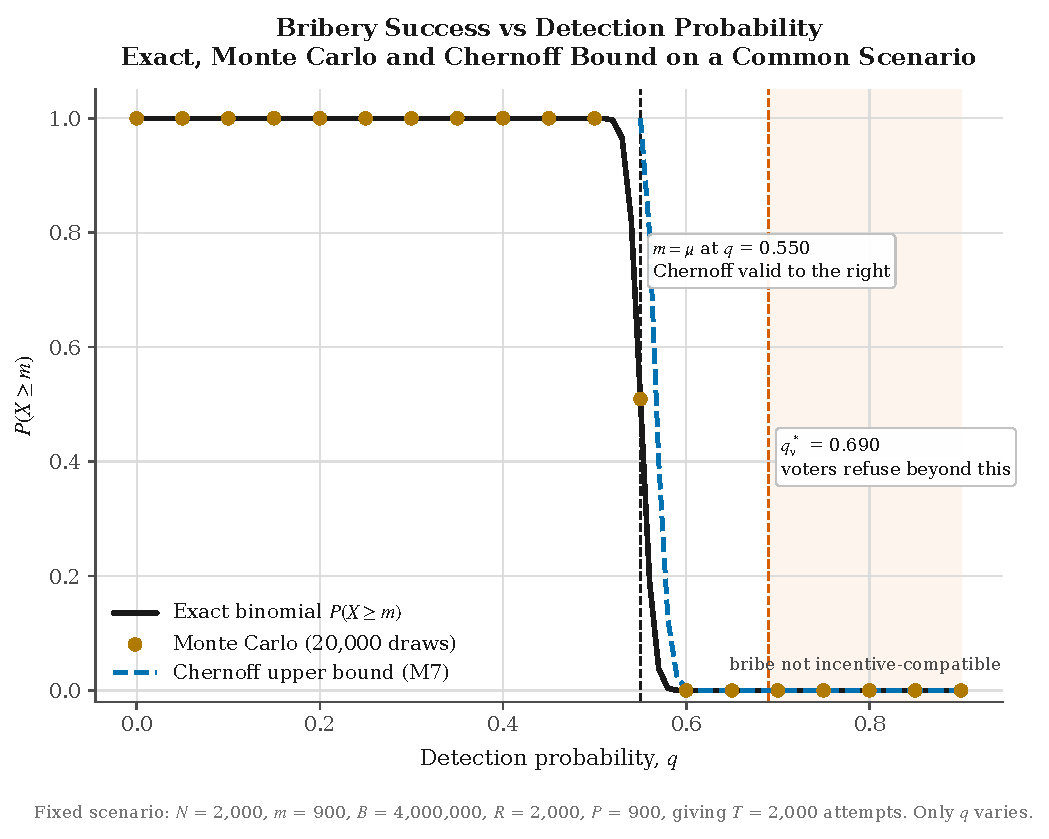
\includegraphics[width=0.92\textwidth]{fig_01_method_comparison.pdf}
\end{figure}

\begin{readbox}
\lookat{One fixed election scenario, with only the detection probability
$q$ varying along the horizontal axis. Three methods compute the same
success probability: the exact binomial calculation (solid black),
a Monte Carlo simulation (gold markers), and the Chernoff upper bound
(dashed blue). The shaded region to the right is where the bribe is no
longer worth accepting.}

\shows{The Monte Carlo estimate is indistinguishable from the exact
curve, and the bound sits above both wherever it is defined --- valid,
but visibly conservative. It also shows the shape of the detection
effect: success stays near certainty and then \emph{collapses} over a
narrow band of $q$, rather than declining steadily.}

\matters{Two things at once. Methodologically, three independent
computations agreeing is strong evidence that none contains an error.
Substantively, the collapse is why detection is the efficient defensive
lever: a small improvement in the right region does far more than a
large improvement anywhere else.}
\end{readbox}

\begin{numberbox}
\keynumber{Mean absolute Monte Carlo error against the exact value:
\BriberyMCError{} for bribery. The simulation and the mathematics agree
to four decimal places.}
\end{numberbox}

%=======================================================================
\clearpage
\section{Why bribery collapses: the voter's decision}

\begin{figure}[H]
\centering
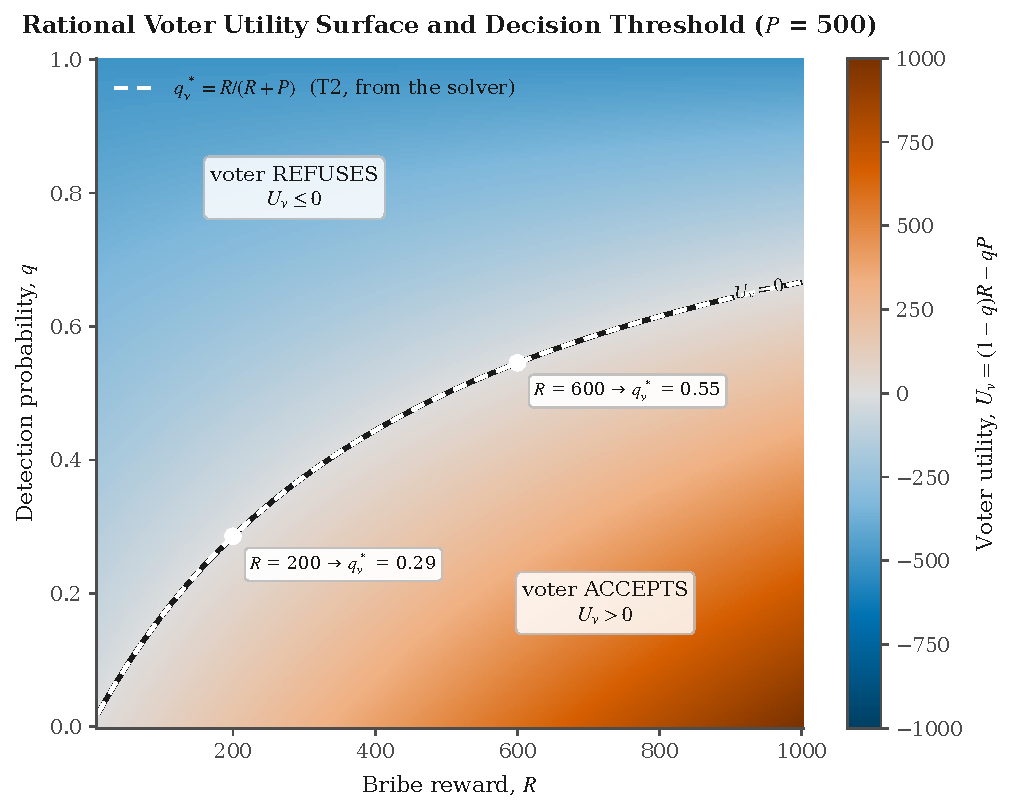
\includegraphics[width=0.86\textwidth]{fig_02_voter_utility_threshold.pdf}
\end{figure}

\begin{readbox}
\lookat{A map of one voter's decision. Left to right is the size of the
bribe offered; bottom to top is the probability of being caught. Warm
colours mean accepting the bribe pays; cool colours mean it does not.
The black curve is the break-even line $\Uv = 0$, and the white dashed
curve is the closed-form threshold $q_v^{*} = R/(R+P)$ drawn on top of
it.}

\shows{Bribery has a consent gate that the other two attacks do not.
Above the threshold curve, a rational voter refuses \emph{any} bribe the
attacker can afford, so the attack stops --- not because fraud was
detected, but because it was never committed. That the numerically
computed boundary and the algebraic formula land on the same curve is
also a check that the solver and the mathematics agree.}

\matters{It explains why bribery behaves discontinuously in every later
figure while Sybil and ballot-stuffing attacks degrade smoothly. Bribery
is suppressed twice --- once by detection, once by refusal --- which is
why it ends up the \emph{least} dangerous of the three vectors under
protection, despite being the one most often discussed.}
\end{readbox}

\begin{numberbox}
\keynumber{$q_v^{*} = R/(R+P)$ depends only on the ratio of bribe to
penalty --- not on the electorate size, the margin, or the attacker's
budget. Raise the penalty and the whole acceptance region shrinks.}
\end{numberbox}

%=======================================================================
\clearpage
\section{Both Chernoff directions validated}

\begin{figure}[H]
\centering
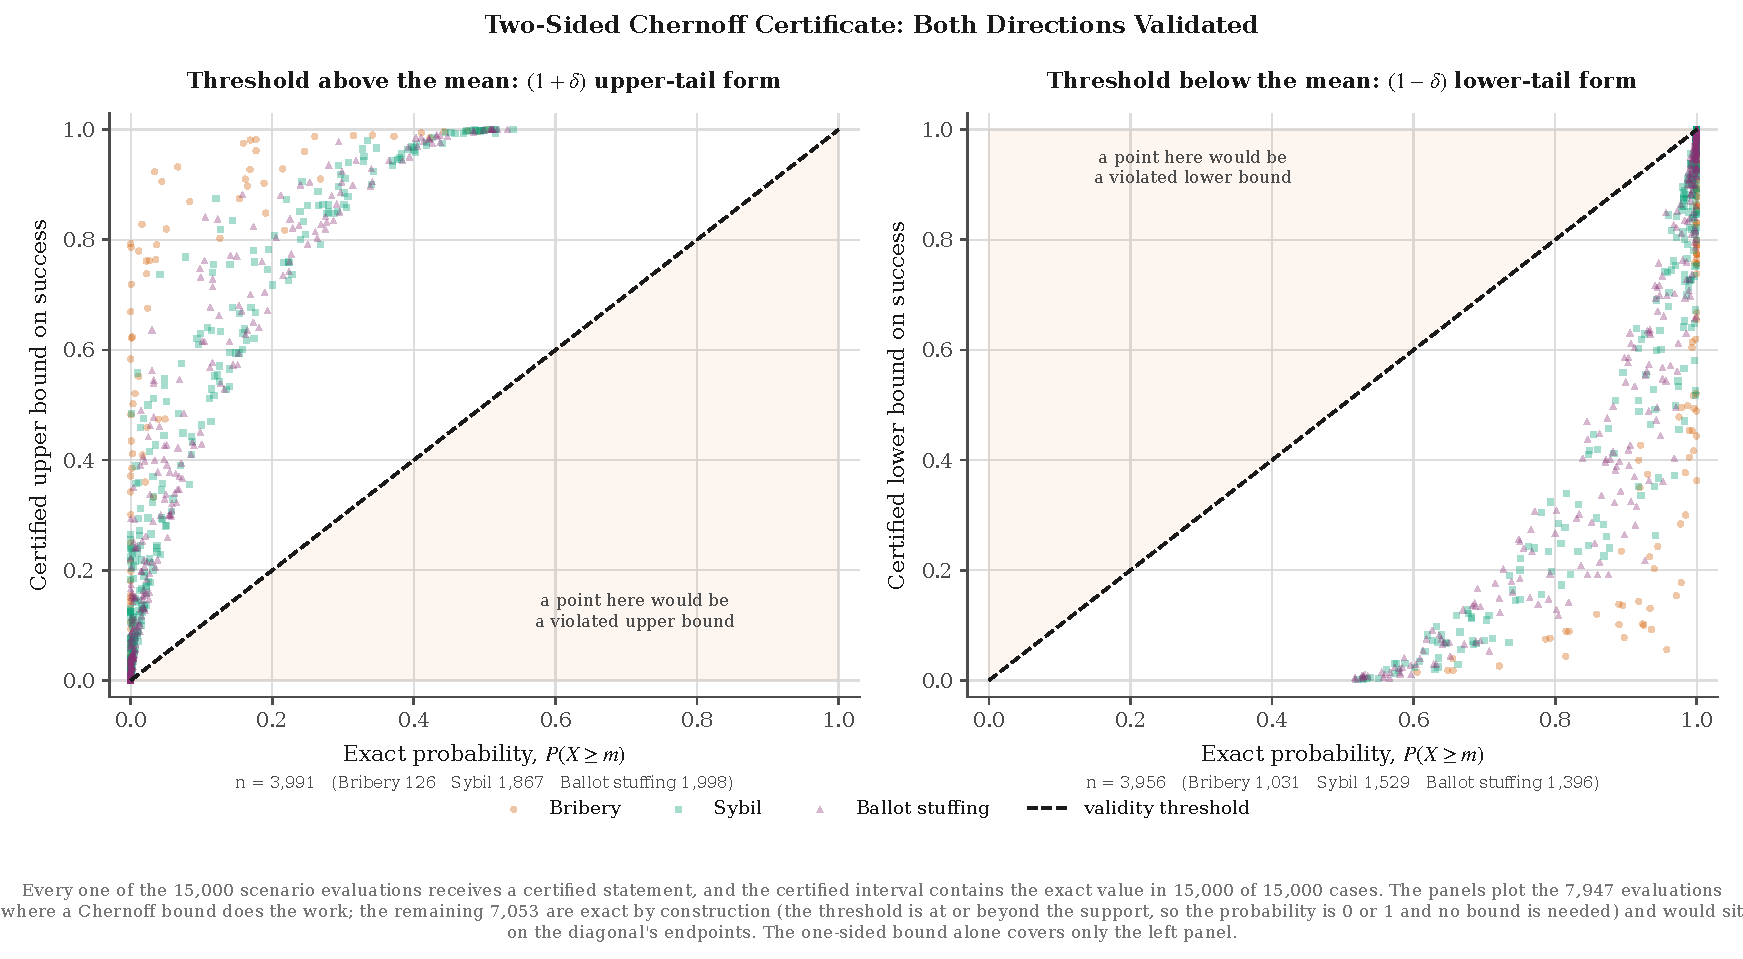
\includegraphics[width=\textwidth]{fig_03_chernoff_two_sided.pdf}
\end{figure}

\begin{readbox}
\lookat{Every scenario in the experiment plotted twice over: its exact
success probability horizontally, and the guarantee proved about it
vertically. Left, where the threshold sits \emph{above} the mean, the
$(1+\delta)$ upper-tail bound certifies success from above, so valid
points lie on or above the diagonal. Right, where the threshold sits
\emph{below} the mean, the $(1-\delta)$ lower-tail form certifies
success from below, so valid points lie on or below it.}

\shows{Both directions hold everywhere. No point falls on the wrong side
of either diagonal. The two forms are not interchangeable --- the factor
records which side of the mean the threshold is on --- and applying
either to the wrong tail produces a statement the data refutes.}

\matters{The one-sided bound alone covers only the left panel, leaving
the scenarios where the attack is \emph{most likely to succeed} with no
proof attached to them at all. Extending to both tails means every
scenario now carries a guarantee, and in the right-hand panel that
guarantee is the stronger kind: not ``the attack cannot exceed this
chance'' but ``the attack succeeds with \emph{at least} this chance''.}
\end{readbox}

\begin{numberbox}
\keynumber{100\% --- the certified interval contains the exact value in
all 15{,}000 scenario evaluations, and none is left without a
statement.}
\end{numberbox}

%=======================================================================
\clearpage
\section{What the countermeasures actually do}

\begin{figure}[H]
\centering
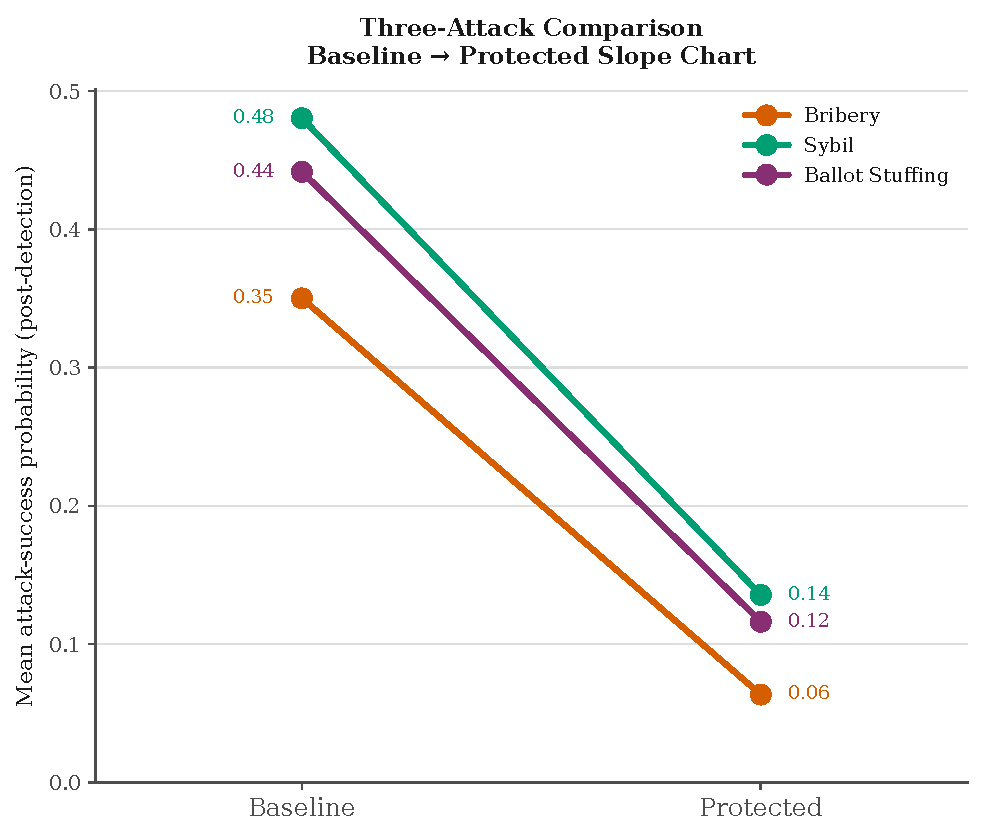
\includegraphics[width=0.78\textwidth]{fig_04_attack_comparison.pdf}
\end{figure}

\begin{readbox}
\lookat{Each line is one attack vector. The left end is its average
success probability against the weakly-defended baseline system; the
right end is the same scenario re-run with blockchain-style audit,
digital signatures, identity verification and ballot validation
switched on. Both ends of every line come from the \emph{same}
\TotalTrials{} scenarios, so the drop is a like-for-like comparison.}

\shows{All three attacks fall sharply --- but not equally. Bribery falls
furthest in relative terms, because it is stopped twice over. Sybil
registration ends up the most resilient vector, retaining roughly twice
the residual success probability of bribery.}

\matters{The ordering is the finding, not the size of the drop. The
weakest link under protection is \emph{identity verification} --- the
one thing a ledger does nothing about. A deployment that hardens the
chain while leaving voter registration weak has hardened the wrong
layer.}
\end{readbox}

\begin{numberbox}
\keynumber{Bribery \BriberyBaseline{} $\rightarrow$ \BriberyProtected{}
(\BriberyRelReduction\%), Sybil \SybilBaseline{} $\rightarrow$
\SybilProtected{} (\SybilRelReduction\%), ballot stuffing
\BallotStuffingBaseline{} $\rightarrow$ \BallotStuffingProtected{}
(\BallotStuffingRelReduction\%).}
\end{numberbox}

%=======================================================================
\clearpage
\section{From probabilities to stolen elections}

\begin{figure}[H]
\centering
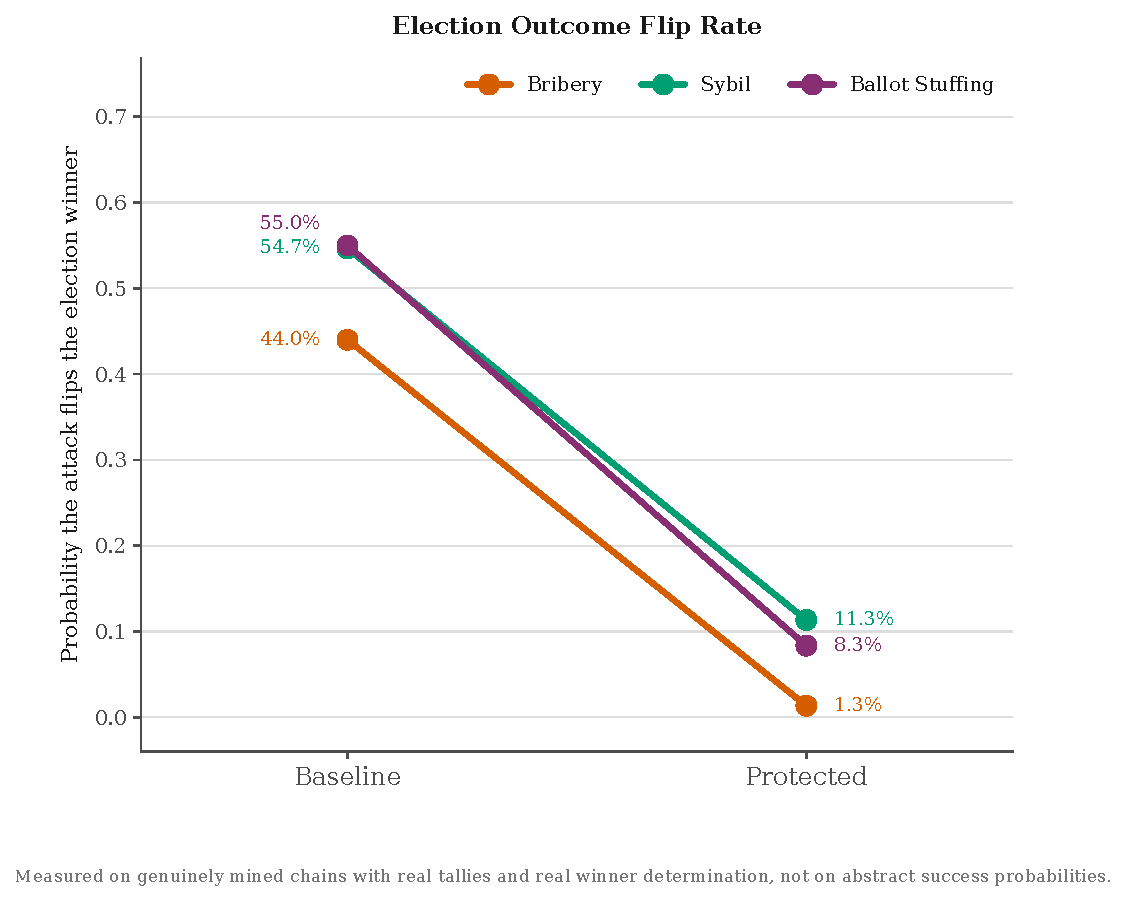
\includegraphics[width=0.76\textwidth]{fig_05_election_flip_rate.pdf}
\end{figure}

\begin{readbox}
\lookat{Not a probability model this time. \ElectionTrials{} elections
were genuinely mined on a proof-of-work blockchain, attacked, and
re-counted from the chain itself to see who actually won. The vertical
axis is the fraction of those elections in which the \emph{winner
changed}.}

\shows{The ordering matches the abstract results exactly, which is the
cross-check the two-layer design exists to provide: an analytic model
and a mined chain, computed independently, agree. Under the baseline
configuration between two and three elections in five were flipped.}

\matters{This is the centrepiece of the dissertation, and it is a
negative result about the technology. The chain's integrity check passed
in \emph{every single trial}, including all the ones where the winner
changed. Every fraudulent vote was correctly formed, correctly mined and
permanently recorded. The ledger did exactly what a ledger is supposed
to do, and the elections were stolen anyway.}
\end{readbox}

\begin{numberbox}
\keynumber{\FlipBriberyBaseline\% of baseline bribery trials flipped the
winner while chain integrity was \ChainIntegrityHeld. Immutability
guarantees a wrong result cannot later be altered --- not that the
result is right.}
\end{numberbox}

%=======================================================================
\clearpage
\section{How much detection is actually needed}

\begin{figure}[H]
\centering
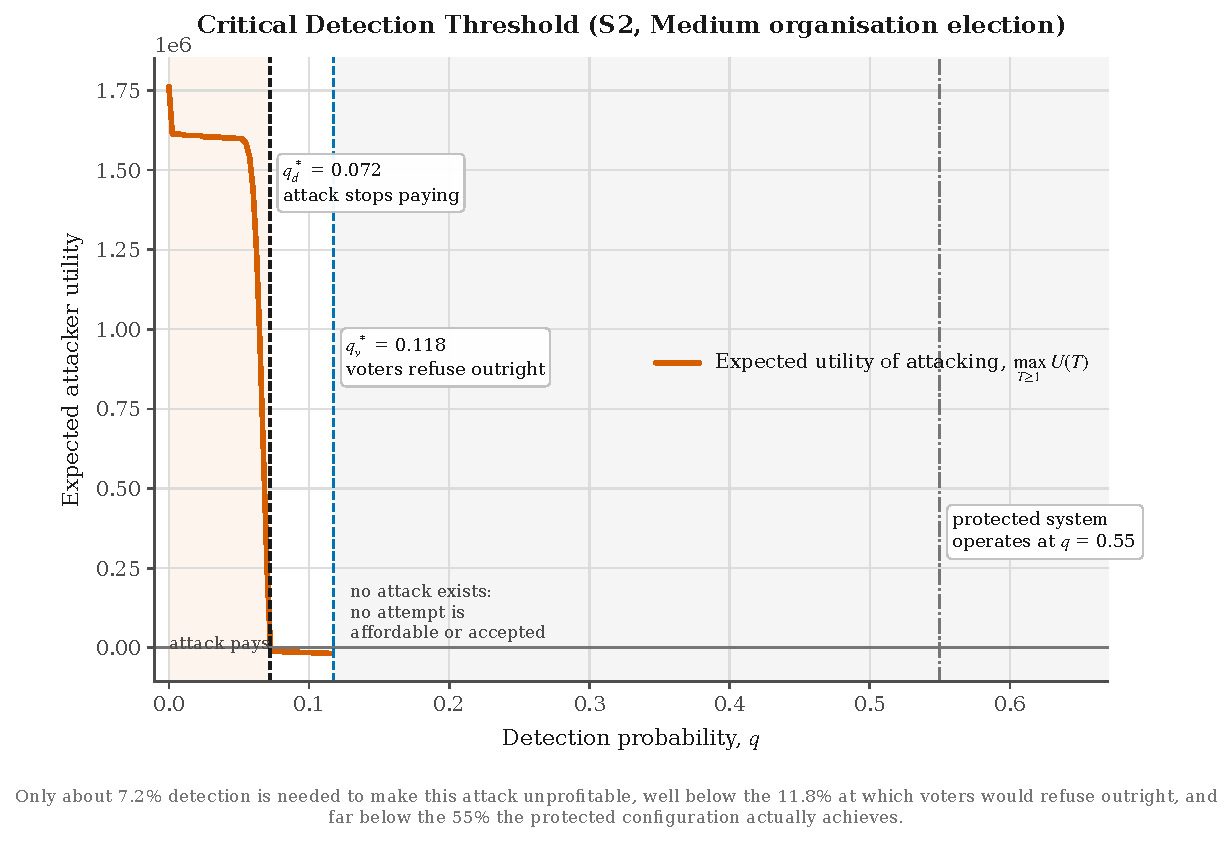
\includegraphics[width=0.88\textwidth]{fig_06_critical_detection.pdf}
\end{figure}

\begin{readbox}
\lookat{The attacker's expected profit as the system's detection
probability improves left to right. The shaded region is where attacking
pays. Three vertical markers: $q_d^{*}$, where profit hits zero and the
attack stops being worth mounting; $q_v^{*}$, where voters refuse
outright and it becomes impossible; and the detection rate the fully
protected system actually delivers.}

\shows{The two thresholds are far apart, and both are far to the left of
what the protected system provides. Between $q_d^{*}$ and $q_v^{*}$ the
attack is still perfectly \emph{possible} --- the budget suffices, the
voters would accept --- but a rational attacker declines because the
expected return has gone negative.}

\matters{This is the most actionable finding in the dissertation, and it
inverts the usual conclusion. The headline result is not that the
countermeasures work; it is that \emph{much weaker ones would have}.
Deterrence arrives long before prevention, and costs far less. The
caveat is that deterrence assumes a rational attacker: someone with
non-monetary motives, or who misjudges the detection rate, is not
deterred by an unfavourable expectation.}
\end{readbox}

\begin{numberbox}
\keynumber{Attacks stop paying at detection probabilities of
\CriticalDetectionMin--\CriticalDetectionMax{} --- roughly
\ProtectionHeadroom$\times$ weaker than the \ProtectedQ{} the protected
system delivers. About one caught bribe in fourteen is enough.}
\end{numberbox}

%=======================================================================
\clearpage
\section{The model in one picture}

\begin{figure}[H]
\centering
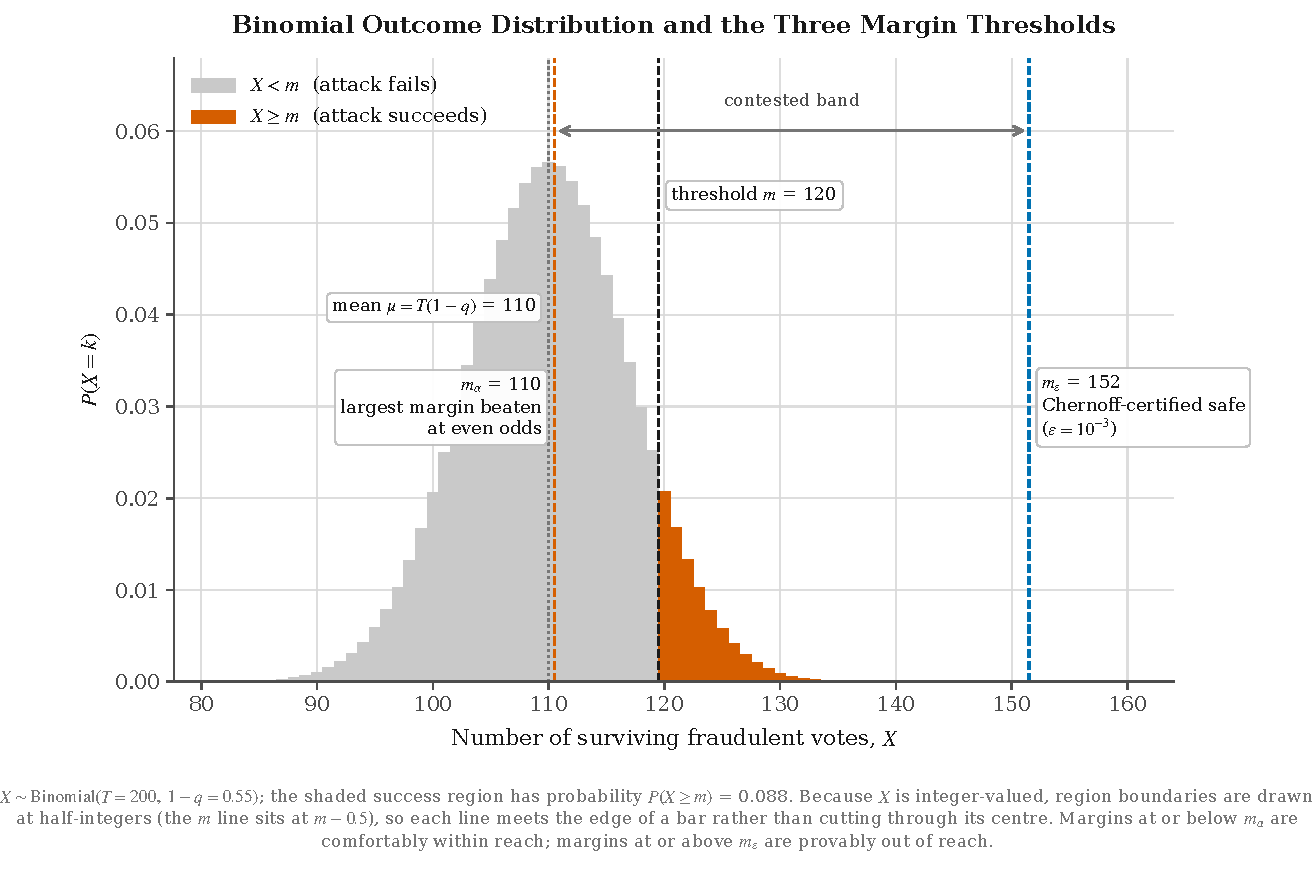
\includegraphics[width=0.94\textwidth]{fig_07_binomial_thresholds.pdf}
\end{figure}

\begin{readbox}
\lookat{The bell-shaped curve is the probability of each possible number
of fraudulent votes surviving the system's defences. The grey bars are
outcomes where the attack \emph{fails}; the vermillion bars are outcomes
where it \emph{succeeds}, because they reach or exceed the manipulation
threshold $m$ --- the number of extra votes needed to overturn the
election. The shaded vermillion area is the attack's success
probability.}

\shows{Attack success is a tail event, not an average. The mean outcome
$\mu$ sits comfortably below the threshold, so a typical attack fails;
the attack succeeds only when the random outcome runs unusually high.
The three labelled thresholds partition the axis: below $m_\alpha$ the
attacker wins at even odds, above $m_\varepsilon$ the Chernoff bound
proves safety, and only the contested band between them needs exact
computation.}

\matters{This one picture defines every number in the dissertation.
``Attack success'' always means reaching $m$ --- never merely that some
fraud occurred, or that it went undetected. It is a deliberately
demanding definition: an attack that injects a hundred fraudulent votes
into an election it fails to flip counts here as a \emph{failure}.}
\end{readbox}

\begin{numberbox}
\keynumber{Margins are safe or contested by a hair. At national scale the
attacker reaches \SThreeMReachable{} votes at even odds while safety is
only provable from \SThreeMCertified{} --- a contested band about 500
votes wide.}
\end{numberbox}

%=======================================================================
\clearpage
\section{The rational attacker does not spend everything}

\begin{figure}[H]
\centering
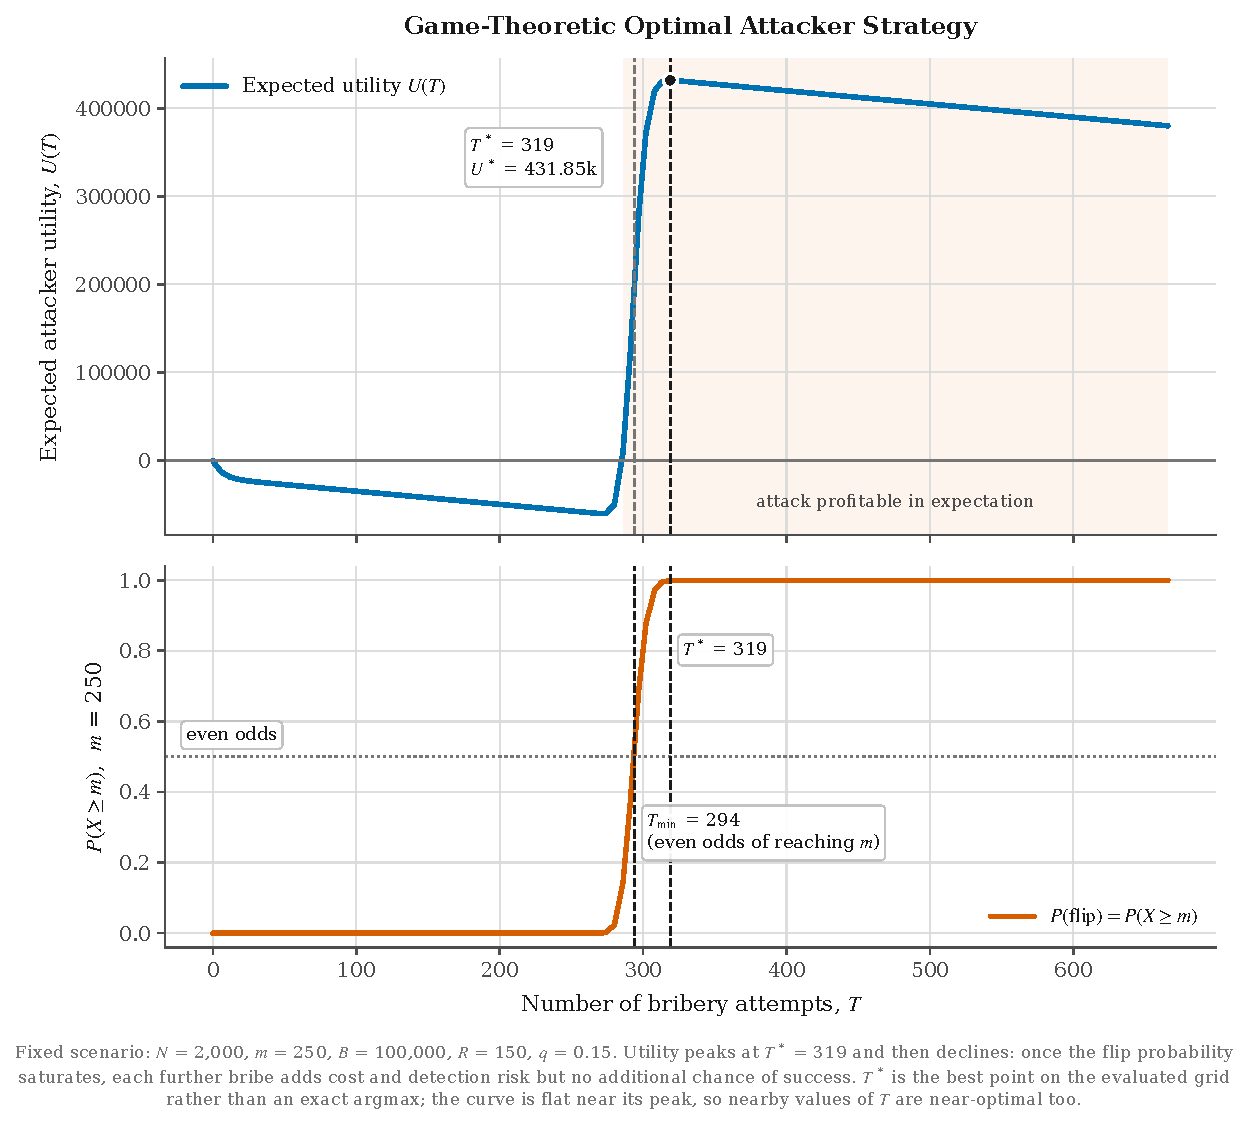
\includegraphics[width=0.86\textwidth]{fig_08_optimal_attacker.pdf}
\end{figure}

\begin{readbox}
\lookat{Two stacked panels sharing a horizontal axis: the number of
bribes the attacker attempts. The top panel is the attacker's expected
profit, the bottom panel is the probability of flipping the election.
$T^{*}$ marks the most profitable strategy, and $T_{\min}$ the effort
needed for an even chance of success.}

\shows{Profit is single-peaked. It rises while extra bribes still move
the flip probability, then \emph{falls} once that probability saturates
near one and every further bribe adds cost and detection risk without
adding any chance of success. Spending the whole budget is a strictly
worse strategy than stopping at $T^{*}$.}

\matters{Security analyses usually assume a maximally-resourced attacker
who spends everything. That attacker is not the dangerous one --- the
dangerous one stops early, spends less, and is harder to notice.
Optimising a defence against maximum expenditure optimises against the
wrong opponent.}
\end{readbox}

\begin{numberbox}
\keynumber{Utility peaks well before the budget is exhausted, and
declines thereafter. The defence question is not ``can they afford it?''
but ``is it worth their while?''}
\end{numberbox}

%=======================================================================
\clearpage
\section{Why no single vector is enough}

\begin{figure}[H]
\centering
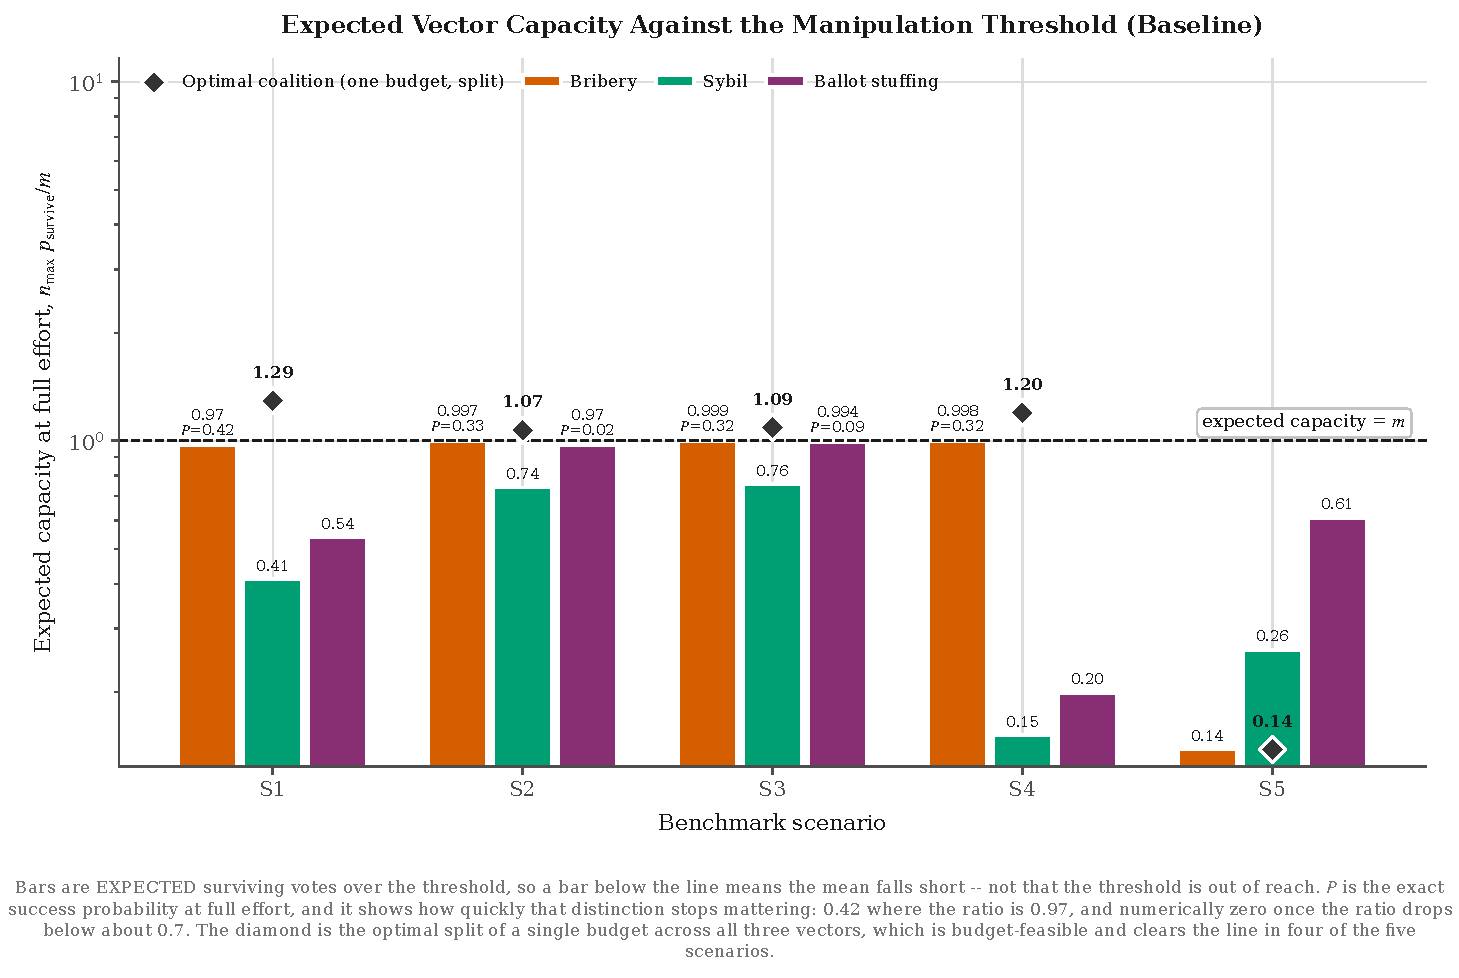
\includegraphics[width=0.94\textwidth]{fig_09_vector_capacity.pdf}
\end{figure}

\begin{readbox}
\lookat{For each benchmark scenario, how many fraudulent votes each
vector could deliver at maximum effort, expressed as a multiple of the
threshold needed to flip the election. The dashed line at 1.0 is that
threshold: a bar reaching it means the vector can win on its own. The
diamond shows all three vectors' capacity added together.}

\shows{Neither Sybil registration nor ballot stuffing reaches the line
in \emph{any} scenario, once realistic limits are respected --- forged
registrations bounded by the registration window, injected ballots
bounded by the turnout figure they would otherwise make implausible.
Individually, two of the three attacks are structurally infeasible. The
combined diamond clears the line comfortably.}

\matters{Read one vector at a time, this is a reassuring result: most of
the attacks cannot work. That reading is wrong, and the next page shows
why. The limits binding each vector are \emph{capacity} limits, and
capacity limits do not add up --- an attacker who spreads effort escapes
all three at once.}
\end{readbox}

\begin{numberbox}
\keynumber{Sybil and ballot stuffing individually reach only
0.14--0.99 of the threshold. Together with bribery they reach
1.01--2.75.}
\end{numberbox}

%=======================================================================
\clearpage
\section{The coalition attack}

\begin{figure}[H]
\centering
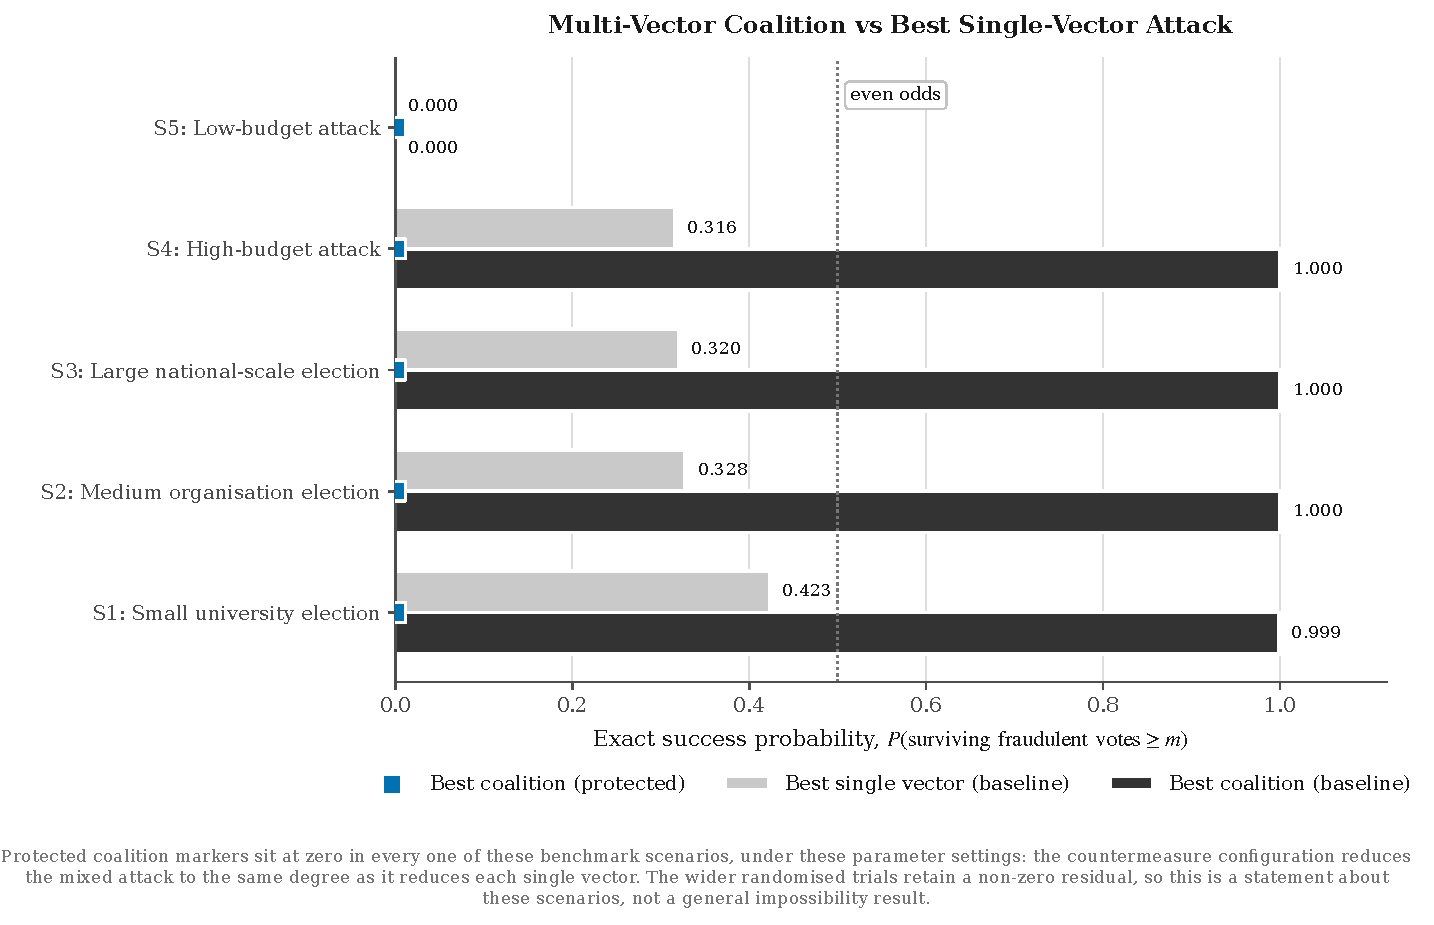
\includegraphics[width=0.94\textwidth]{fig_10_coalition_vs_pure.pdf}
\end{figure}

\begin{readbox}
\lookat{For each scenario, two bars and a marker. The grey bar is the
best the attacker can do committing the whole budget to a single
vector; the dark bar is the best achievable by splitting that same
budget across all three at once. The blue square is the mixed attack
re-run against the protected system.}

\shows{Mixing wins, and not by a little. In the high-budget scenario no
single vector exceeds a success probability of \SFourExactFlip{}, yet
the mixture reaches near-certainty. The mechanism is capacity, not
probability: each vector saturates its own ceiling long before the money
runs out, and the leftover budget buys nothing more there but a great
deal elsewhere.}

\matters{Evaluating attack vectors one at a time is \emph{not} the
conservative choice it appears to be. Doing so here would have declared
the attack infeasible when in fact it succeeds decisively. The
reassuring news is that the same countermeasures still hold: every
protected marker sits at zero.}
\end{readbox}

\begin{numberbox}
\keynumber{The mixed strategy beats the best single vector in
\CoalitionBetterCount{} of \CoalitionScenarioCount{} scenarios, lifting
mean success from \BestPureMeanBaseline{} to \CoalitionMeanBaseline{}
--- and the result survives all \SensitivityConfigs{} cost
configurations tested.}
\end{numberbox}

%=======================================================================
\clearpage
\section*{The argument in six sentences}
\addcontentsline{toc}{section}{The argument in six sentences}

\begin{enumerate}[leftmargin=1.6em,itemsep=5pt]
\item An attack succeeds only if enough fraudulent votes survive every
      defence to overturn the margin, which makes election security a
      question about a probability distribution rather than a binary
      vulnerability.
\item Bribery is stopped by voters refusing as much as by detection,
      which is why it ends up the least dangerous of the three vectors
      once defences are switched on.
\item Three independent computational methods --- exact, simulated and
      proved --- agree everywhere they are all defined, and the proved
      bound now covers both tails, so every scenario carries a
      guarantee.
\item The modelled countermeasures cut attack success by
      \SybilRelReduction--\BriberyRelReduction\%, but the residual risk
      concentrates in identity verification, which is precisely what a
      ledger does not address.
\item Chain integrity held in every one of \ElectionTrials{} mined
      elections, and \FlipBriberyBaseline\% of the baseline ones were
      stolen regardless --- immutability and correctness are different
      properties.
\item Making an attack unprofitable takes roughly
      \ProtectionHeadroom$\times$ less detection than making it
      impossible, and an attacker who combines vectors beats one who
      commits to the best single vector in
      \CoalitionBetterCount{} of \CoalitionScenarioCount{} scenarios ---
      so defenders should buy deterrence first, and should never
      evaluate attack vectors in isolation.
\end{enumerate}

\vfill
{\footnotesize\color{inkmuted}
The full dissertation, including the literature review, the formal
model, the methodology and all thirty figures, is available separately.
Every number in this summary is injected at build time from the
simulation output and is reproducible from seed \Seed.}

\end{document}
